
\begin{frame}
\frametitle{Networking}
\begin{itemize}
\item Networking is about communication
\item Text is the simplest way to communicate
\item Protocols are standards for reading and writing text
\end{itemize}
\tiny
\href{https://betterexplained.com/articles/a-simple-introduction-to-computer-networking/}{Ref.}
\normalsize
\end{frame}


\begin{frame}
\frametitle{Networking}
To communicate we must identify the players.\\

Someone's phone number or the address.
\begin{center}
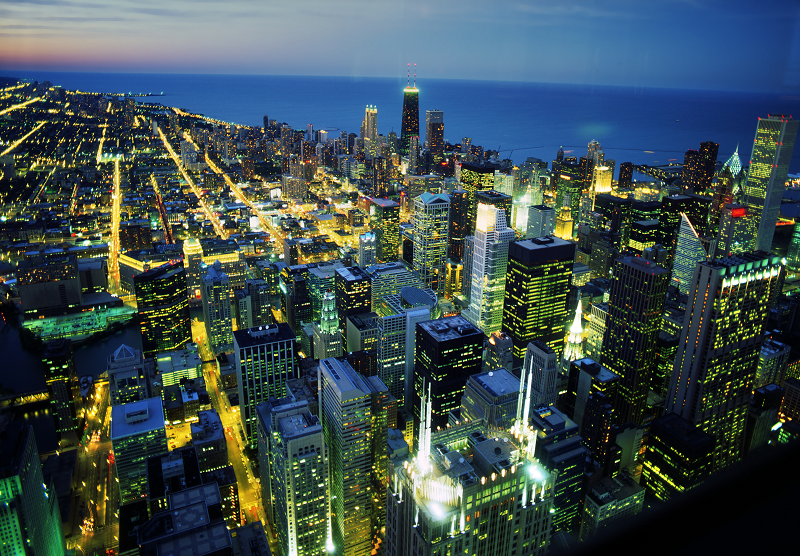
\includegraphics[width=\columnwidth]{./Figure/network/ChicagovanafSearsTower}
\end{center}
\end{frame}


\begin{frame}
\frametitle{Networking}
To communicate we must identify the players.\\

Now the internal door number
\begin{center}
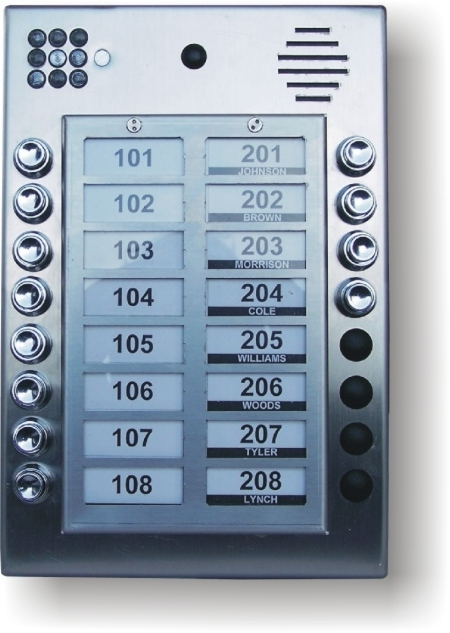
\includegraphics[width=4cm]{./Figure/network/BellGuard_Front_small}
\end{center}
\end{frame}


\begin{frame}
\frametitle{Networking}
To communicate we must identify the players.\\

\begin{columns}
\begin{column}{0.5\textwidth}
\begin{center}
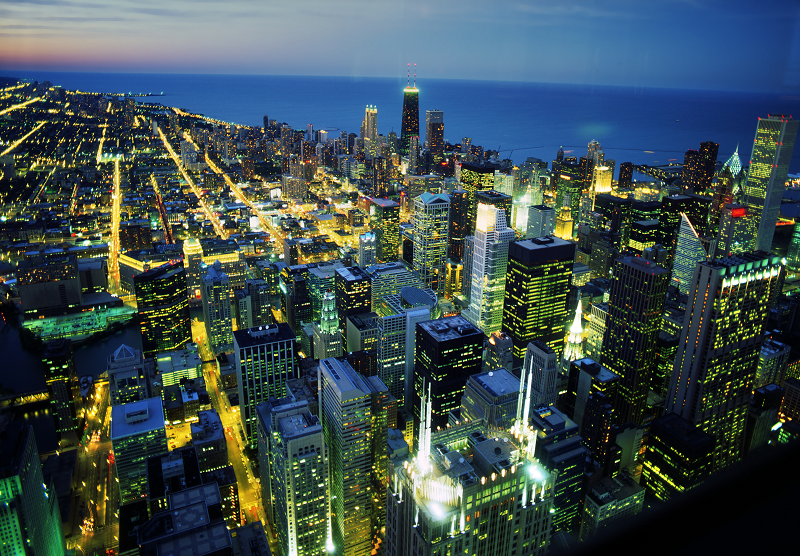
\includegraphics[width=4cm]{./Figure/network/ChicagovanafSearsTower}\\
IP
\end{center}
\end{column}
\begin{column}{0.5\textwidth}
\begin{center}
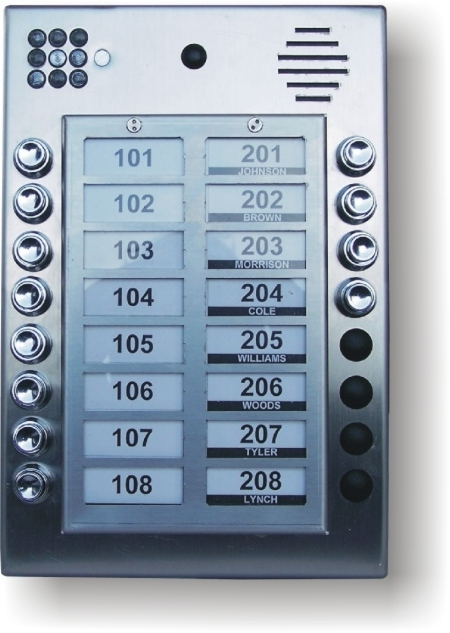
\includegraphics[width=4cm]{./Figure/network/BellGuard_Front_small}\\
PORT
\end{center}
\end{column}
\end{columns}
\end{frame}

\begin{frame}[fragile]
\frametitle{Networking}
A computer is identified by an \textit{IP} number:
\begin{lstlisting}
127.0.0.1

10.0.2.5

172.29.10.1

192.168.1.1
\end{lstlisting}
\end{frame}

\begin{frame}[fragile]
\frametitle{Networking}
IPs can span multiple rangers
\begin{lstlisting}
10.0.0.0 - 10.255.255.255

172.16.0.0 - 172.31.255.255

192.168.0.0 - 192.168.255.255
\end{lstlisting}
\end{frame}

\begin{frame}
\frametitle{Networking}
Usually an IP corresponds to a single network card.
\end{frame}

\begin{frame}
\frametitle{Networking}
WiFi is a radio network card so has an IP.
\end{frame}




\begin{frame}
\frametitle{Networking}
\begin{itemize}
\item Networking is about communication
\item Text is the simplest way to communicate
\item Protocols are standards for reading and writing text
\item Ports are channels from which communications pass-thought
\end{itemize}
\tiny
\href{https://betterexplained.com/articles/a-simple-introduction-to-computer-networking/}{Ref.}
\normalsize
\end{frame}

